%   Template for applications for observing time at ESO/MPG 2.2m-telescope
%
%          Original version January 01, 2008 (H.-J. Roeser}
%          This version: April 2011
%
%            requires ESO22.sty
%
%
%   ************************************************************
%   * This template contains explicit instructions as to how   *
%   * to fill in the LaTeX-commands (comments + examples).     *
%   *                                                          *
%   *       Please follow these instructions carefully!        *
%   *                                                          *
%   * Since this LaTeX-file is automatically analysed to       *
%   * collect the statistical information and prepare the      *
%   * applications for the referees you must not manipulate    *
%   * this file (e.g. omit or permutate commands).             *
%   * Do not concatenate two commands into one line!           *
%   * Commands not needed have to be supplied with an empty    *
%   * argument (e.g. \SchedulingConstraints{} ).               *
%   ************************************************************
%
%  General Information:
%
%  Only proposals written in English are accepted!
%
%  The Style-File and the Template-File were tested with LaTeX 2e
%  (Version 2000/06/01) or TeX-Version 3.14159.
%
%  To create an empty form, empty calls {} have to be selected.
%
%  Comments always refer to the argument or group of arguments
%  of the  *** PREVIOUS *** line.
%
%  Forced linebreaks (\\ or empty line) do not work with most commands.
%  Please use the command \newline instead!
%
%  Type size and page format must not be changed, especially
%  not within the scientific justification!
%  The given number of pages and arrangement are checked! If your pages
%  overflow the space provided, a LaTeX-error will occur.
%
%  The list of publications and the citations from the scientific
%  justification can (but do not have to) be created by LaTeX-command
%  \cite{label} (see item publications). A mixture of manual entries
%  and the use of \cite{label}, though, is not possible.
%
%  Some frequent symbols are defined in the style-file:
%     \etal \privcom \eg \ie \ibidem \dito
%
%  Units for math-mode (in rm-Font)
%     \GHz \MHz \Hz \pc \kpc \Mpc \cm \sec \Kelvin \Jy \mJy \microJy
%
%====================================================================
%
\documentclass[a4paper]{article}
\usepackage[pdftex]{graphicx}
\usepackage{ifthen}
\usepackage{ESO22}
\usepackage{latexsym}
\DeclareGraphicsExtensions{.pdf}    % file extension for images
%\graphicspath{{figures/}}          % optional path to image files
%
\begin{document}
%
% ========================== p a g e  1 =============================
%
%                     Group, from which the application originates
%                     Comment/uncomment as appropriate
%
\MPIAapplication      % MPIA
%\MPGapplication%      % MPG institute other than MPIA
%\OTHER                % all others
%
\ApplicationPeriod{October 2015}  %  e.g.  October 2011
\TelTwoPointTwo{}{}   % {flag}{proposal reference ID of previous proposal}
%
% -------------------------------------------------------------------
%                         Types of applications
% -------------------------------------------------------------------
%
% The type of your application - if applicable - is specified in
% the above command for the telescope selection as the 1. argument,
% perhaps together with the reference number of the previously
% submitted application as a 2. argument. If none of the cases
% described below is applicable, leave both arguments empty.
%
% Long term projects (> 2 semesters): P, L
% ========================================
% Applications for PhD thesis work and long projects may be flagged,
% PhD thesis with a P, other long term projects with an L in the 1.
% argument to the telescope call above. If this flag is used, for both
% an additional page (item 8e) has to be filled in below, describing
% the current / planned logistics of the project. Is this an application
% to continue observations from previous semesters, please quote the
% reference number of the former application in the 2. argument.
%
% The purpose of flagging PhD programs is to request a particularly
% thorough initial application with an outline of all anticipated
% observations. In return, PhD programs can then usually expect
% subsequent approval within the framework of the initial request,
% as long as a satisfactory update on the PhD student's progress
% is provided in subsequent applications. Such a bonus will, however,
% not be given for long-term projects, which have to compete again fully
% with all other proposals currently submitted. For the latter the
% flag is intended to help the referees judging the overall project
% and its needs.
%
% Repetitive applications: W, T, C, R
% ===================================
% If a previous run has been lost due to weather or technical problems,
% the re-submitted proposal should be flagged. W indicates loss due to
% weather, T due to technical difficulties. Indicate the reference
% number of the previous application in the 2. argument.
% If you re-submit an application to continue a project (less than 3
% semesters in total duration) you may flag it with an C. Re-submission
% of a previously rejected application may be flagged with an R. Both
% should include the reference number of the former application in the
% 2. argument.
%
% Example:
% \TelTwoPointTwo{C}{Oct07 #64} is a re-submission of an application
% analogous to application #64 in October 2007 period.
%
% ---------------------------------------------------------------------
%
\Applicant{Dr}{Melissa}{Ness}
        % Title Name Surname of the principal investigator (P.I.)
        %             ( =addressee of correspondence)
{MPIA}
        % Institute
{K\"onigstuhl}
        % Street
{69117}{Heidelberg}
        % ZIP-code Town
{mkness}
        % ESO User Portal username
{ness@mpia.de}
        % complete e-mail address
%
\Collaborators{\small Casey, Kennedy, Hartle, Irwin, Gilmore}{University of Cambridge}
        % collaborators: Name(s)  Institute(s)
{Schlaufman}{Carnegie Observatories}
        %                Name(s)  Institute(s)
       
\Observers{A. Casey}
           {M. Ness/G.Kennedy}
        % Name(s) of the applicants/collaborators who will
        % perform the observation.
\Category{E}    % category
        % Please choose ONE category that comes closest to your
        % application by giving the corresponding letter
        % in the argument.
        %
        % A = Cosmology, intergalactic medium,
        %     clusters of galaxies, galaxies
        % B = active galactic nuclei
        % C = interstellar medium, star formation, milky way
        % D = massive / hot stars
        % E = low-mass / cold stars
        % F = solar system
        % G = instrumentation
\Title{Awakening the Giants}

        % Only one line!
\Abstract{
The bulge and disc host the most red giant branch (RGB) stars in the Galaxy. Current photometric selections of disk/bulge stars are heavily contaminated by nearby, uninformative main sequence stars. Our program uses a unique photometric selection to isolate RGB tracers of the Milky Way's formation. We request 9 nights to obtain narrow-band imaging across 200~deg$^2$ in the bulge. When combined with public g- \& K-band photometry, we can select FGK RGB stars with 1\% contamination (compared to $\sim$30\%) and $\sim$90\% completeness. RGB star metallicities are linearly correlated with mid-infrared colours, enabling precise stellar parameter estimates from photometry. This program will enable the most efficient search for Population III stars, and vastly improve APOGEE-2's bulge target selection.
}
%and will vastly improve APOGEE-2's bulge target selection.
        % The length of the abstract must not change the page layout!
\Instrument{WFI}   % WFI  or  FEROS  or  GROND
%
\FluxLevel{$\sim$8}    % from
          {20}    % to
          {V-mag}    % unit of measurement of the brightness given
                %  (e.g. K-mag, Jy at 660nm or similar)
%
% The following information has to contain the SUM of the time
% applied for as a (real) number (e.g. 3.5 or 0.2) to facilitate
% the electronic processing of the data.
% Further details (e.g. 3 x 1/2 night) are to be specified under
% item 11 with the command \SchedulingConstraints !
%
\Hours{} % no restriction  % number of hours applied for
      {} % grey            %       (without weather corrections!)
      {9} % dark            %     please specify only ONE of these!
      {} % already awarded for this project (leave empty if none).
      {9} % hours expectedly needed to finish this project,
         %        in addition to the present application.
         %   ----> leave empty if you do not intend to submit further
         %         proposals in future semesters for this project.
         % Only integer/real numbers (no blanks, no LaTeX-code) !
%
\ObsTimeRange{30.07.2016}{08.08.2016}
        % best date range for observations {from} {to}
        % Format to ease electronic processing: dd.mm.yy (no blanks !)
        %
        % examples:
        %  {1..10.10}{31.3.11}  i.e. no limit in P88
        %  {1.2.11}{15.4.11}    i.e. beginning Feb. - mid-Apr. 2011
        %
        % Any scheduling constraints should be given under item 11.
\LST{14:00}{22:00}
%       Optimum range in local sideral time (LST) in hours {from}{to}
%       Format to ease electronic processing: hh:mm
%                 (e.g. {5:30}{10:00}, no blanks allowed!)
%
% ========================== p a g e  2 =============================
%
\begin{ObservingProgram}
%
%  Scientific justification
%  A maximum of 1 page text (no changes to font size should be made!)
%  An additional page is at your disposal for pictures and tables to
%  support your application!
%
%  Please describe the following:
%
%     -- outline of astrophysical problem
%     -- scientific aim of the observations and what the novelty is,
%     -- own previous work in this context,
%     -- layout of the observation.
%
%  In the last point please explain specifically how the
%  observations planned will lead to the projected aim, i.e. the
%  answer to the scientific questions.
%
%  For long-term projects, nights allocated thus far have to be given
%  (item 13) as well as the number of nights needed to finish the
%  programme (item 6). Especially the results reached so far have to
%  be presented under item 8.
%
%  When wording your application, please take into consideration the
%  following: Our committee is small (compared to HST's or ESO's).
%  Its is, therefore, evident that we do not always have a specialist
%  for each and every small area of interest.
%  For this reason you should present aim and previous work in such a
%  way that any experienced astrophysicist can follow your arguments
%  (e.g. do not use unusual abbreviations, known to only a chosen few).
%  Papers not yet published should be handed in as preprints. As there
%  is a large number of applications to be surveyed it is unreasonable
%  to have to consult the web to be able to understand the background
%  and previous work of an application! Reference to papers in preprint-
%  servers, therefore, is pointless.
%
\subsection*{Astrophysical context}
% outline of astrophysical problem

The bulge and disc contain the largest numbers of stellar tracers of the Milky Way and therefore host the most information content about the Galaxy's formation and evolution.  For this reason numerous spectroscopic studies have sought to survey red giant branch (RGB) stars in the plane of the Milky Way.  However these observations are challenging: stellar crowding, strong absolute and differential extinction all negatively impact the photometric target selection.  This results in a relatively high fraction ($\sim$30\% or higher) of nearby dwarf stars that contaminate the sample.  If RGB stars could be robustly selected from photometry, and their stellar parameters ($T_{\rm eff}$, $\log{g}$, ${\rm [Fe/H]}$) could be reliably estimated without the need for spectroscopy, this would reveal rare objects with high scientific impact (e.g., low-mass metal-free Population III stars, of which none have been discovered) as well as enabling high-level inferences about the chemical evolution of the Milky Way.


\subsection*{Immediate aim}
%scientific aim of the observations and what the novelty is,

We propose to obtain narrow-band imaging at 510~nm in the bulge to enable the most efficient photometric selection of RGB stars ever constructed.  We utilise data from the \textit{Kepler} field to demonstrate the efficiency and effectiveness of our proposed observations.  The \textit{Kepler} field has been extensively imaged in multiple filters (broad- and narrow-band), with numerous spectroscopic studies reporting stellar parameters, providing a uniquely unbiased sample with which to construct our photometric selection. One  filter employed was the narrow-band $DDO_{51}$ filter centered at $\sim$510~nm (Giesler, 1984). This filter includes the MgH molecular feature (present only in dwarf stars) and the strong Mg I b triplet lines. The Mg triplet lines saturate quickly, producing absorption profiles with extensive wings induced by pressure broadening. Because the broad-band $g$ filter peaks near the same central wavelength as $DDO_{51}$ (Fig. 1), the $g-DDO_{51}$ colour is extremely sensitive to photospheric pressure (and therefore surface gravity $\log{g}$), with little dependence on spectral type.  This is clearly demonstrated in Fig. 2, where a simple colour cut in $g-K_s$ (a $T_{\rm eff}$ proxy) and $g - DDO_{51}$ (green area) yields a robust selection of giant stars ($\sim$90\% completeness) with negligible dwarf contamination ($\sim$1\%).  Our simple selection function outperforms any existing photometric selection for RGB stars.  Moreover, because the two filters peak at the same wavelength, the $g-DDO_{51}$ colour is minimally affected by extinction. 

The resulting selection of RGB stars have metallicities that linearly correlate with mid-infrared colours (Fig. 3). This allows us to precisely estimate stellar parameters ($T_{\rm eff}$, [Fe/H], and therefore $\log{g}$) of every RGB star towards the bulge, without the need for expensive spectroscopy. 

% When our proposed narrow-band imaging data is combined with existing public optical and mid-infrared photometry, these data will highlight superlative objects (e.g., metal-free Population III stars), permit high-level inferences about the chemical evolution of the disc and bulge, and provide a legacy catalog for planned spectroscopic surveys in the Milky Way plane (e.g., APOGEE-2).


\subsection*{Previous work}
Our team are expert and uniquely suited to this programme.  Ness is an expert on using stellar metallicities and kinematics to reveal signatures of formation in the bulge (Ness et al. 2012,2013ab,2014ab).  Schlaufman \& Casey (2014) presented a novel, efficient selection of EMP stars that uses only public, all-sky near- and mid-infrared photometry to identify metal-poor star candidates due to their lack of molecular absorption near 4.6 microns. Their selection has identified the most metal-poor stars currently in the bulge, which likely formed at $z > 10$ and are chemically distinct from comparable halo metal-poor stars (Casey \& Schlaufman, 2015). Recently, Hartle, Kennedy \& Casey have refined the photometric selection presented here using \textit{Kepler} data, which motivates this proposal. Irwin, as director of the Cambridge Astronomical Survey Unit, is an expert in data reduction and is a co-investigator on the VPHAS Survey.


\subsection*{Layout of observations}
Our proposed observations are strategically matched to leverage existing ESO/VPHAS $g$-band and GLIMPSE mid-infrared data. The existing $g$-band imaging will simplify the WFI$_{871}$ photometry (e.g., forced photometry using an existing catalog) and provide stellar $\log{g}$ sensitivity through the $g-WFI_{871}$ colour. GLIMPSE data exists for all planned observations, and the $IRAC_{1} - IRAC_{2}$ colour (see Fig. 3) permits estimates of stellar metallicity.  The planned VPHAS Survey area is shown in Fig. 4, including the existing $g$-band imaging released in Data Release 2, and our planned observations. This proposal is timely: VPHAS $g$-band imaging for most of our proposed observations will be released in Data Release 3 in mid-2016. Nevertheless, we will prioritise fields with existing public $g$-band data.


\subsection*{Strategic importance for MPIA}
MPIA is an institutional member of APOGEE, and the southern complement APOGEE-2. Both surveys obtain infrared spectra for candidate RGB stars. These data would provide a robust, reproducible selection of RGB candidates that could potentially maximise the scientific yield of APOGEE-2 in the bulge, and further MPIA's critical involvement in the SDSS collaboration. 

We note that although \textit{Gaia} will deliver stellar parameter estimates from BP/RP and parallaxes, these will only be available in the final data release ($\sim$2022, after APOGEE-2). Additionally, due to the crowded nature of the bulge and limited bandwidth, it is likely that most stars will not have sufficiently high S/N in BP/RP spectra to robustly determine stellar parameters.  Thus, we request a modest amount of small telescope time to enable this novel, high-impact science and enhance MPIA's involvement in APOGEE-2.

\end{ObservingProgram}
%
% ========================== p a g e  3 =============================
%
% This page is only for pictures and tables in support of the
% application. It must not be used for additional text!
%
% The following lines give an example of how to insert a single-column
% picture. Pictures that expand over both columns can be inserted
% likewise, with only the caption remaining single-column. When using
% the LaTeX-commando \begin{figure*} allowing a two-column caption,
% unfortunately an unwanted page-break occurs.
% Therefore please do not use this feature!
%
%
\begin{SupportingMaterial}

\begin{figure}
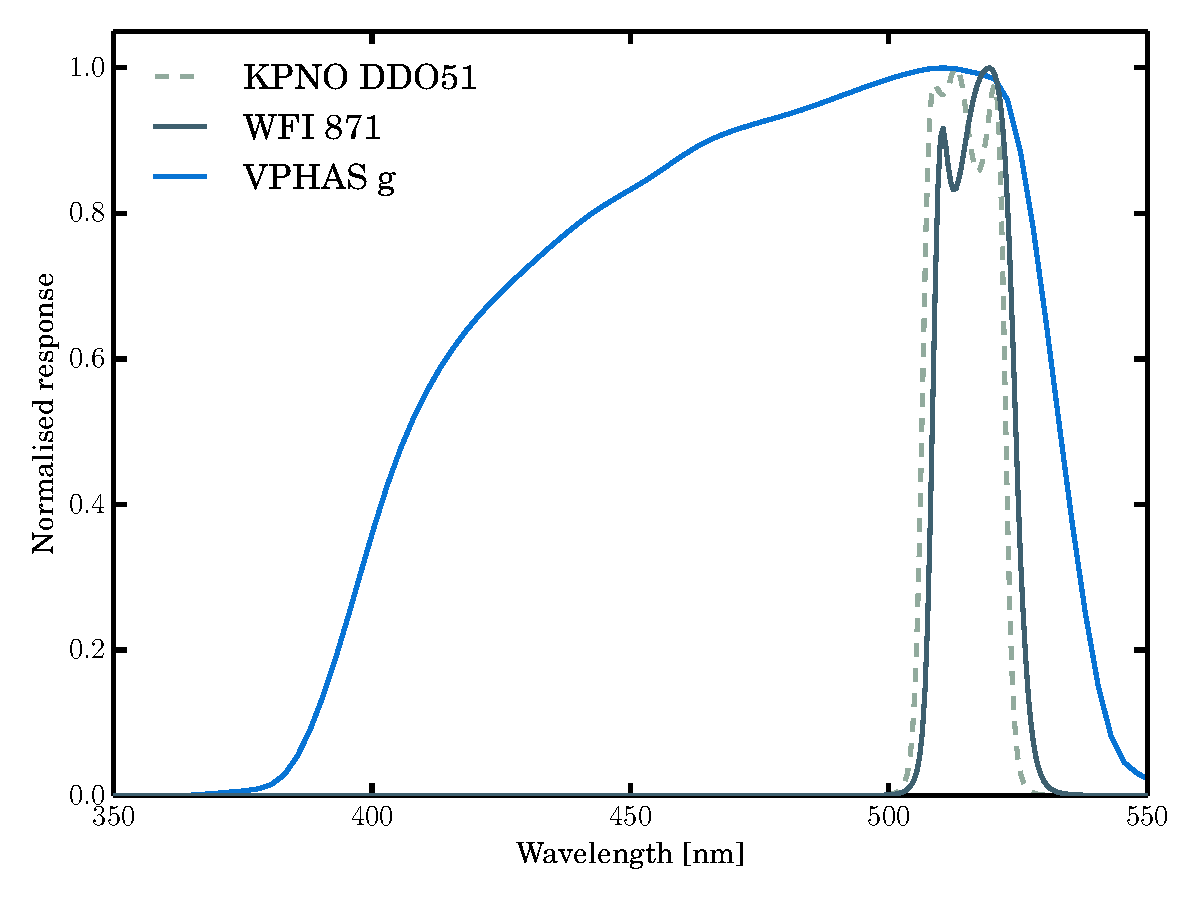
\includegraphics[width=8.3cm,angle=0,clip=true]{filter-response}
\caption{\label{image1} The relative system response curve for the $DDO_{51}$ (dashed), VPHAS $g$ (blue), and WFI 871 (grey) filters. The $DDO_{51}$ filter includes pressure-sensitive absorption lines in stellar spectra (see text), making the $g-DDO_{51}$ colour extremely sensitive to stellar surface gravity $\log{g}$. Only two $DDO_{51}$ filters exist, both in the northern hemisphere, and neither are suitably sized for any southern imaging telescope. However, this figure demonstrates that the response of the WFI 871 filter is analogous to $DDO_{51}$.}
\end{figure}


\begin{figure}
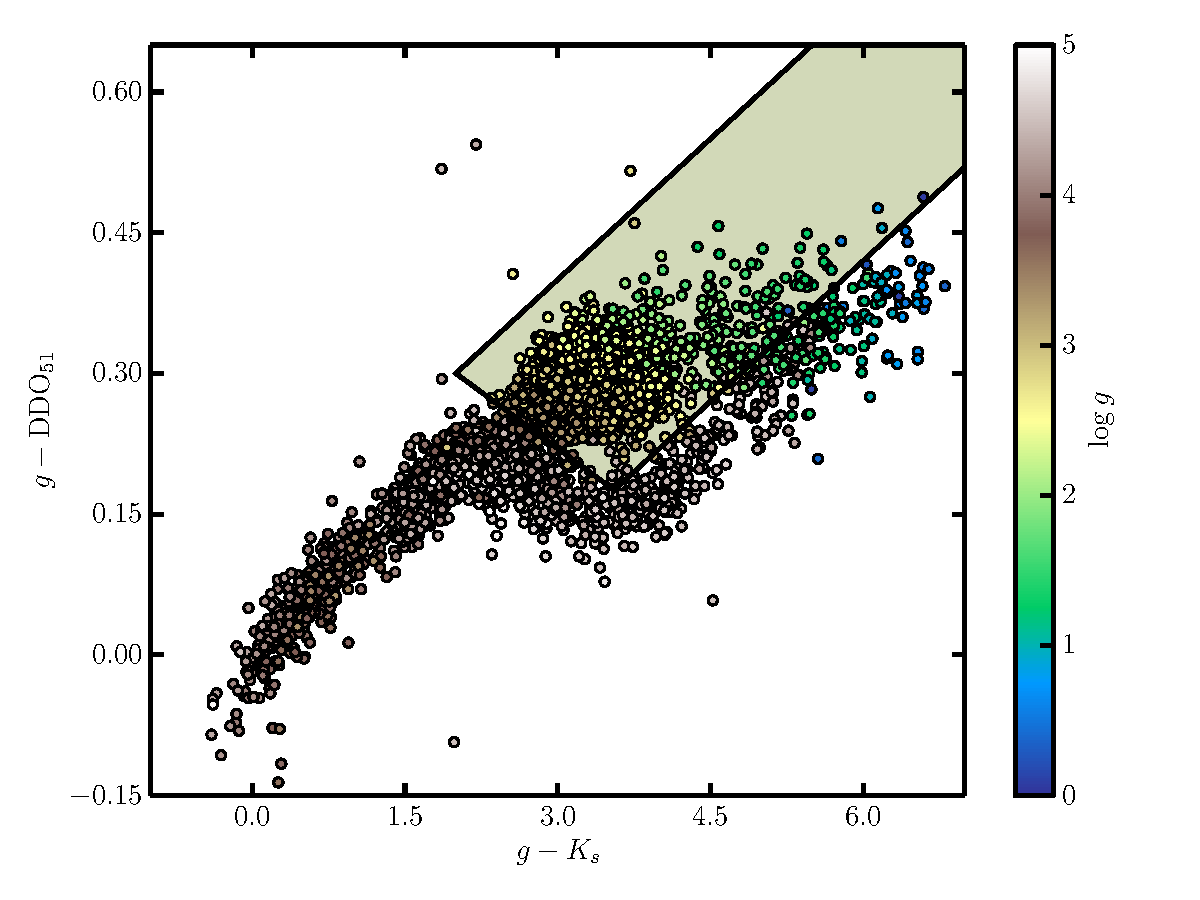
\includegraphics[width=8.3cm,angle=0,clip=true]{giant-selection}
\caption{\label{image2} \textit{Kepler} field stars with $g-K_s$ (a proxy for $T_{\rm eff}$) and $g-DDO_{51}$ photometric colours. Each point is coloured by surface gravities spectroscopically determined by LAMOST, demonstrating that $g-DDO_{51}$ clearly separates giant and dwarf stars. A simple (easily invertible) colour selection box is shown by the green region, yielding 90\% completeness of RGB stars with just 1\% contamination.}
\end{figure}



\begin{figure}[t!]
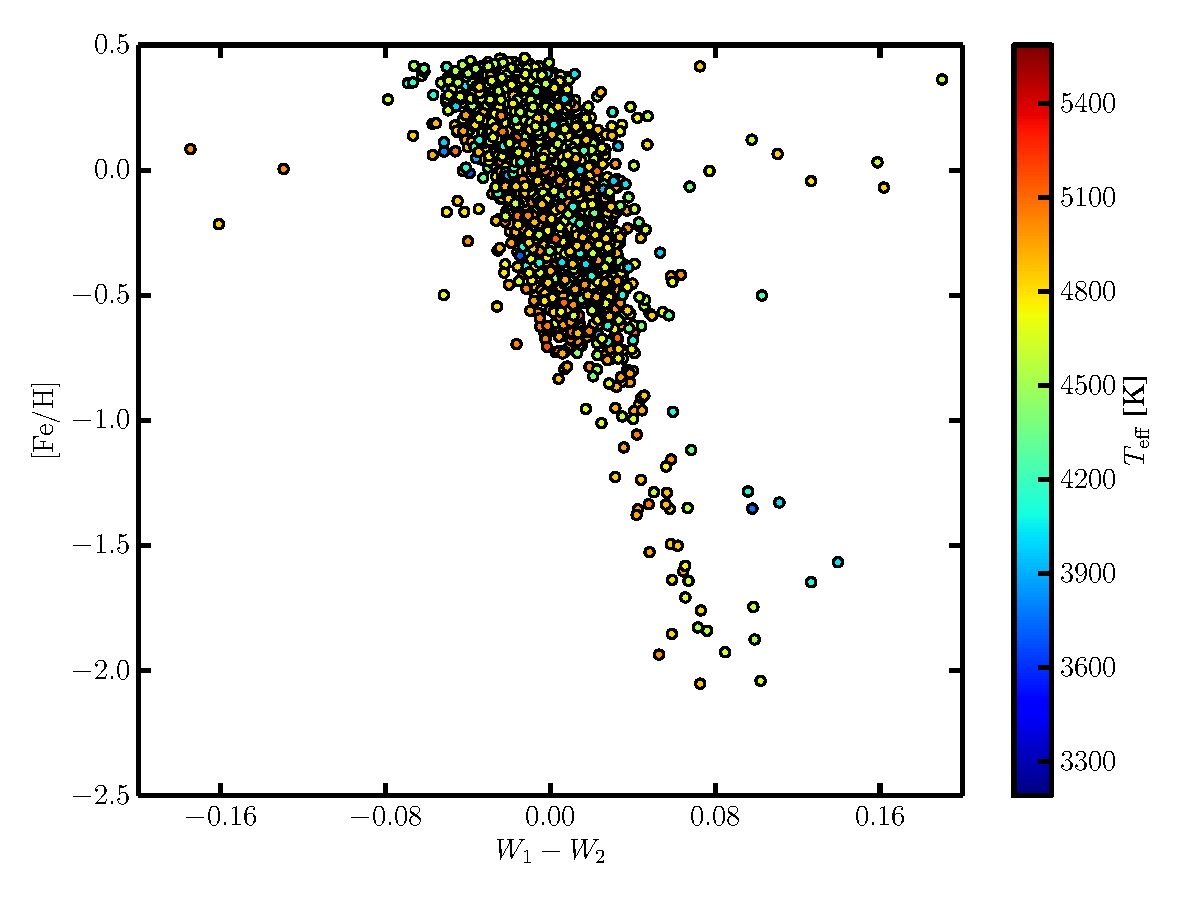
\includegraphics[width=8.3cm,angle=0,clip=true]{wise-metallicity}
\caption{\label{image3}The mid-infrared WISE colour $W_1 - W_2$ (corrected for $T_{\rm eff}$ effects) against stellar metallicity for the RGB star sample selected in Figure 2. Stellar metallicity is linearly correlated with $W_1 - W_2$ due to strong molecular absorption at 4.6 microns. No residual correlation is seen with $T_{\rm eff}$, allowing precise estimates of stellar parameters and the most efficient selection of extremely metal-poor stars ever constructed. Due to the large point spread function of WISE data, our bulge survey will use the public GLIMPSE $IRAC_1 -  IRAC_2$ colour, which covers the same wavelengths as $W_1 - W_2$.}
\end{figure}


\begin{figure}
%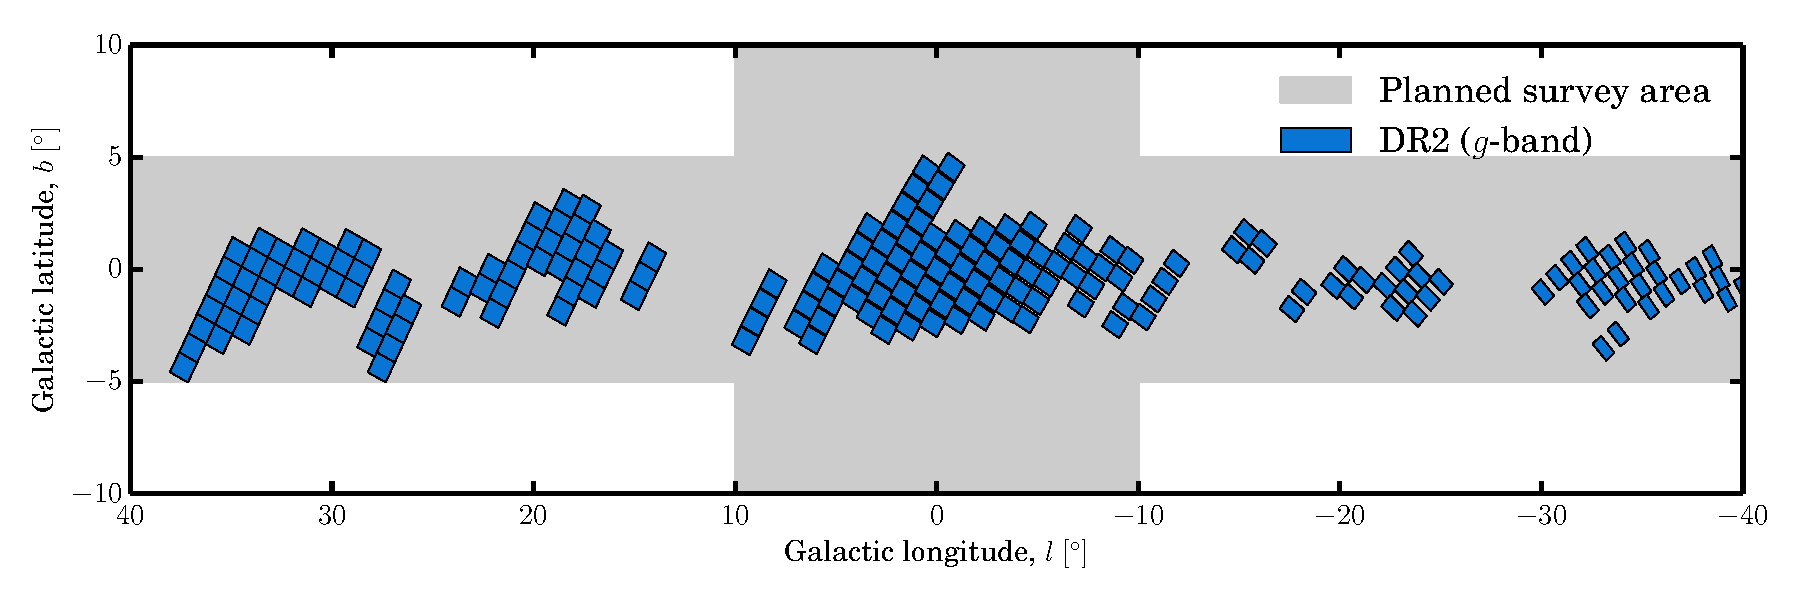
\includegraphics[width=\textwidth,angle=0,clip=true]{vphas-g}
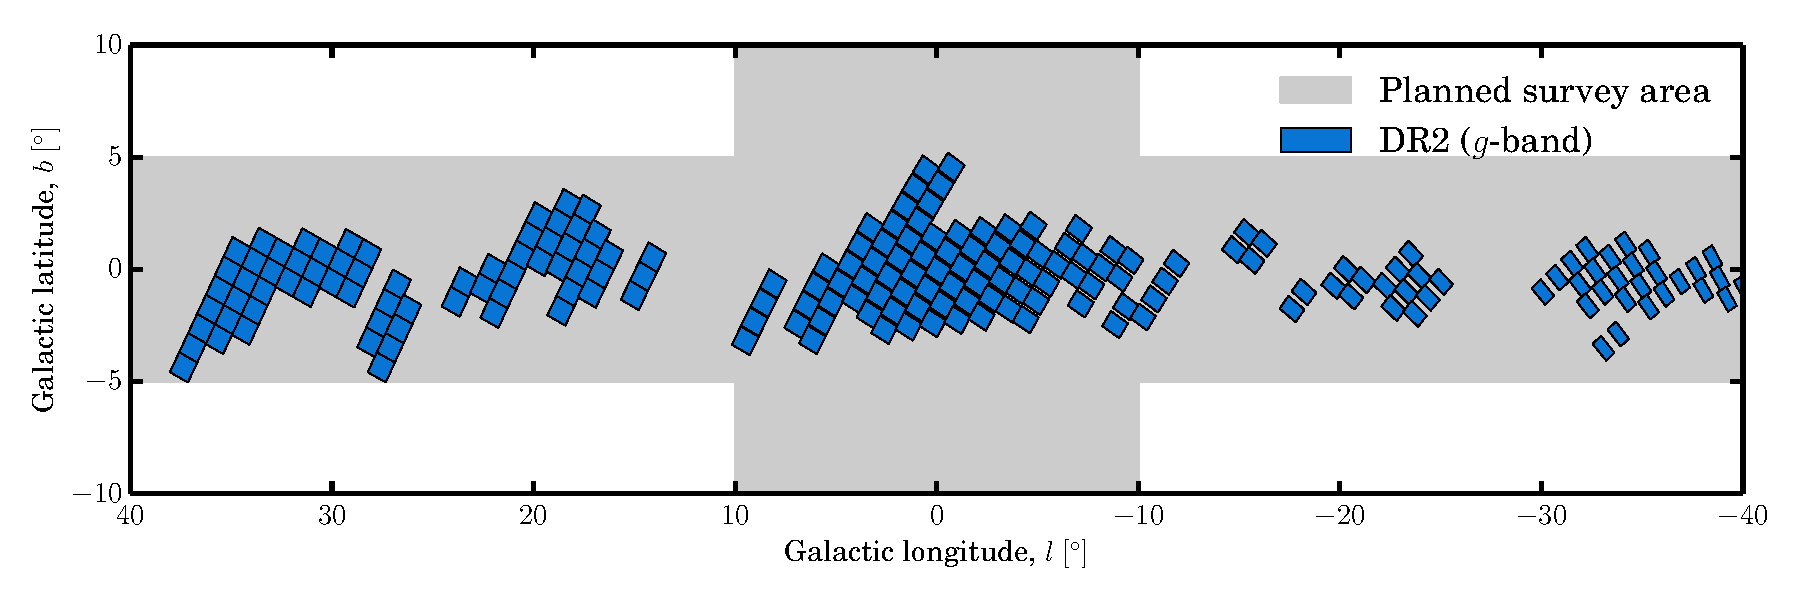
\includegraphics[width=8.3cm,angle=0,clip=true]{vphas-g}
\caption{\label{image4}Galactic coordinates ($l, b$) showing the existing coverage of the VPHAS $g$-band imaging (Data Release 2; blue), and the planned survey area for VPHAS. We will complement our narrow-band imaging with public VPHAS $g$-band data. The area including our proposed observations are marked, which will be released by VPHAS in Data Release 3 prior to our scheduled observations.}
\end{figure}

\end{SupportingMaterial}


%
% ========================== p a g e  3a =============================
%
% Backup project:
% Projects with special observing requirements (exceptionally good
% seeing, photometric conditions etc.) have to present a fully
% adequate backup programme.
%
% The same comments as under item 8 above are applicable.
%
%\begin{BackupProgramm}
%\subsection*{Astrophysical context}
%\subsection*{Immediate aim}
%\subsection*{Previous work}
%\subsection*{Layout of observations}
%\end{BackupProgramm}
%
% ========================== p a g e  3b =============================
%
% This page is only for pictures and tables supporting the
% backup programme. It must not be used for additional text!
%
%\begin{BackupSupportingMaterial}
%\begin{figure}
%\includegraphics[width=8.3cm,angle=0,clip=true]{image1}
%\caption{\label{image1}}
%\end{figure}
%\end{BackupSupportingMaterial}
%
% ========================== p a g e  3c ===========================
%
% Description of the current logistics for
%                      PhD thesis work and long term projects
%
%\begin{Logistics}
%
%\end{Logistics}
%
% ========================== p a g e  4 ==============================
%
% If you wish to use a different heading instead of the brightness in
% the 4th column of the object table below (something more
% characteristic for your application, e.g. the redshift) you may
% change the text of the column-heading via the command
%   \def\HeadLine{new heading}, e.g.
%   \def\HeadLine{redshift\newline of the  QSOs},
% which you insert here (before the \begin{Targets} command).
%
%\def\HeadLine{}
%
\begin{Targets}
%
%--------------------------------------------------------------------
%  List only those objects scheduled for observation during the span
%  of time applied for.
%  Pay attention to observability and good use of the night!
%  If one page is not sufficient, name only representative objects.
%--------------------------------------------------------------------
%
% Examples of format
%        (footnotes to the table are possible with \footnote{}):
%
% Name & \RA{h}{m}{s}{fract s} & \DEC{d}{'}{"} & mag & priority \\
%      & \RA{}{}{}{} & \DEC{}{}{} & & \\
%
Bulge & \RA{18}{00}{00}{00} & \DEC{-30}{00}{00} & $\sim$8-20 & High \\
\end{Targets}
%
% ========================== p a g e  5 =============================
%
\TimeJustification{
The ESO exposure time calculator for the WFI reveals that 100 seconds of integration time is required to acquire $S/N \sim 25$ for K2V-type star with $V = 20$ at airmass $1.2$ in 0.8\arcsec seeing in dark conditions (3 days from new moon). Because our observations are in the blue and very sensitive to scattered light, we require dark conditions. We conservatively estimate $\sim$3 minutes of overheads per field, totalling 5 minutes per field. Our planned survey area totals 200~deg$^2$, requiring $\sim$800 fields. The bulge is accessible (airmass $<$ 1.5) from La Silla for 8 hours/night in June/July. Therefore we require 9 nights to complete our proposed observations.
}
%       Justification for the amount of time applied for.
%       Please indicate also why this special telescope/
%       instrument is needed or particularly suitable.
%
\SchedulingConstraints{The PI and many co-Is will likely be attending the Cool Stars conference in Uppsala on 1-6 June, 2016.
}
%       Leave empty if there are no restrictions.
%
%       Otherwise, give the constraints and/or restrictions
%       which are important for scheduling your observations.
%       Please be brief here!
%       Examples:
%               Before 3.5m-observations !
%               Not between ... and ... !
%               Simultaneously to HST-observations at ... !
%
\ObsExperience{Ness has observed for 5 nights on DECAM, $>$15 nights on AAT/AAOmega.

Casey has more than 30 nights of commissioning experience with SkyMapper, and has observed with the following spectroscopic telescope/instrument combinations: VLT/FLAMES (6 nights), Keck/DEIMOS (1 n), Magellan/MIKE ($>$15 n), KPNO Mayall/Echelle (3 n), AAT/AAOmega (17 n), ANU 2.3/WiFeS (3 n).}
%       Observational experience regarding the project applied for
%
\begin{Publications}
            % Results and publications of campaigns during
            % the past three years in form of a table (see example).
            % ***** Please remain within the given format ******
            % In the last column indicate the corresponding
            % reference under item 14 and there under item
            % \BibliographieListen in argument #2 list the full
            % quotation (including title).
            %
            % With the optional command \StatusOfProjects a short
            % summary of projects carried out during the last years at
            % the ESO2.2m may be added to the table in support of this
            % application.
            %
% Columns of table:
% Telescope & instrument & period & hours & success [%] & publications
% Example:
%  2.2m     &   FEROS    &  Jul 05  &   25  &   85\%  & \cite{CA-2}\\
%\StatusOfProjects{}
%
\end{Publications}
%
%
% ========================== p a g e  6 =============================
%
\BibliographyLists{manual}{
Geisler (1984): {\em Luminosity classification with the Washington system}, PASP, {\bf 96}, 723 \\
Ness, Freeman, Athanassoula, et al. (2012): {\em The Origin of the Split Red Clump in the Galactic Bulge of the Milky Way}, ApJ, {\bf 756}, 22 \\
Ness, Freeman, Athanassoula, et al. (2013a): {\em ARGOS - III. Stellar populations in the Galactic bulge of the Milky Way}, MNRAS, {\bf 430}, 836 \\
Ness, Freeman, Athanassoula, et al. (2013b): {\em ARGOS - IV. The kinematics of the Milky Way bulge}, MNRAS, {\bf 432}, 2092 \\
Ness, Debattista, Bensby, et al. (2014a): {\em Young Stars in an Old Bulge: A Natural Outcome of Internal Evolution in the Milky Way}, ApJ, {\bf 787}, 19 \\
Ness, Aspund, Casey (2014b): {\em NGC 6522: a typical globular cluster in the Galactic bulge without signatures of rapidly rotating Population III stars}, MNRAS, {\bf 445}, 2994 \\
Schlaufman \& Casey (2014): {\em The Best and Brightest Metal-poor Stars}, ApJ, {\bf 797}, 13 \\
Casey \& Schlaufman (2015): {\em Chemistry of the Most Metal-poor Stars in the Bulge and the $z > 10$ Universe}, ApJ, {\bf 809}, 110 \\
}{}
%\BibliographyLists{manuell}{}{}
%
% ------------------------------------------------------------------
% The bibliographical details in argument 2 and 3 of this call above
% refer to item 8 resp. 13 of the application.
%
% If as first argument {auto} is used, all references within the
% text are carried out via LaTeX-command \cite{label}. The references
% have then to be given as second and third argument as follows:
%
% 2. argument =
%      references relating to scientific justification (item 8):
%{\bibitem{label}{reference}
% \bibitem{label}{reference}
%    ...
%}{
% These two brackets separate the 2nd and 3rd argument.
% 3. argument =
%      references to past observations on Calar Alto (item 13):
%\bibitem{label}{reference}
%\bibitem{label}{reference}
%    ...
%}%  closes 3rd argument
%
% When using the Auto-Modus the entries to (8) receive
% consecutive numbers <100, those to (13) numbers >99.
%
% Example:
%
% If the text gives: "... produces  $H_0=10$ \cite{Mei76} ...",
% insert in the 2. argument of \BibliographyLists the following:
% {    ...
%\bibitem{Mei76}{Meier (1976): {\em The Hubble-constant},
%        A\&A {\bf 123}, 1024}
%      ...    }
%
% If the references are inserted manually into the text and the
% literature list is formatted manually, the call has to be as
% follows:
%
%\BibliographyLists{manual}{references to 8}{references to 13}
%
% In this case the applicant has to take care of the necessary
% cross-references himself. The information under item 8 will
% automatically be separated by a horizontal line from those
% under item 13.
%
% Example:
%\BibliographyLists{manual}%
%{Meier (1976): {\em the Hubble-constant}, A\&A {\bf 123}, 1024\\
% Schmidt (1963): {\em Identification of 3C\,273}, Nature {\bf 197}, 10
%}{Ich (1997): {\em the XYZ-constant}, ApJ {\bf 123}, 987\\
% Ich und Du (1998): {\em Die Entfernung zu M\,31}, PASP {\bf 145}, 12}
%
% A T T E N T I O N:
% ================
%
% A mixture of the two modi in the arguments 2 und 3 is not possible!
% That is either  ** ALL **  citations (in the scientific justification
% as well as those papers going back to observations with the ESO2.2m) are
% done by \cite{mark} or ** ALL **  citations and references are
% inserted manually.
%
% ========================== p a g e  7 =============================
%
\MinimumObservingRequirements
        {1.5}  % worst tolerable seeing ["],  e.g. {2.5}
        {50}  % minimum transparency [%],  e.g. {50}
        {1.5}  % maximum airmass,  e.g. {1.5}
        {yes}  % photometric conditions required [yes/no]
        {0.3/90} % maximum moon phase [0-1 in units of illuminated fraction]
            %   / min. distance to object [degrees],  e.g. {0.8/30}
        {/} % min./max. time difference between individual observations
            %   in case of service observation [days/days], e.g. {2/10}
\EndOfApplication


